I hope to have found something by this point in the thesis.

%% $Id$
%
%Although the upper limit that we have placed on the rate of binary black hole
%MACHO inspirals in the galaxy is lower than the upper bound of the predicted
%rates, the LIGO interferometers were not at design sensitivity when the S2
%data was taken. At present, the sensitivities of the instruments are
%significantly better than during S2, as can be seen from
%figure~\ref{f:s3strain}, and progress on reducing noise in the interferometers
%continues apace.  The increase in detector sensitivity makes a larger volume
%of the Universe accessible to searches for binary inspirals. In addition to
%this, the amount of data is also increasing as the interferometers become more
%stable.
%
%These improvements in the instruments will increase the chance of detecting
%gravitational waves from binary inspirals. If the rates of binary black hole
%MACHO coalescence are truly as high as predicted, then initial LIGO would
%stand an excellent chance of detecting an inspiral. The first detection of
%gravitational waves will be a major scientific breakthrough and will yield and
%enormous amount of scientific information, particularly if the detection came
%from a binary black hole MACHO. The length of binary black hole MACHO
%inspirals in the sensitive band of the interferometer will allow extremely
%accurate parameter estimation as well as tests of post-Newtonian theory. For
%systems with total mass greater than $\sim 0.64\,\mathrm{M}_\odot$ LIGO will
%be sensitive to the coalescence of the binary and will be able to study the
%strong gravitational field effects when two binary black holes merge. When
%this is coupled with the accurate parameter estimation available from the
%earlier part of the waveform, the inspiral of a binary black hole MACHO could
%be an excellent laboratory for General Relativity.  A detection would also
%impact the studies of halo dark matter and early universe physics, providing a
%MACHO component to the halo and suggesting that primordial black holes do
%indeed form in the universe.
%
%In the absence of detection, the improvements in detector sensitivity will
%dramatically improve the upper limits placed on the rate of binary black hole
%MACHO inspirals. Once these rates are below the predicted rates, we may begin
%to use observations from gravitational wave interferometers to constrain the
%fraction of galactic halos in the form of primordial black hole MACHOs. While
%this may not be as significant as a detection, it will still be of interest to
%the astrophysical community.
%
%\newpage 
%
%\begin{figure}[p]
%\vspace{5pt}
%\begin{center}
%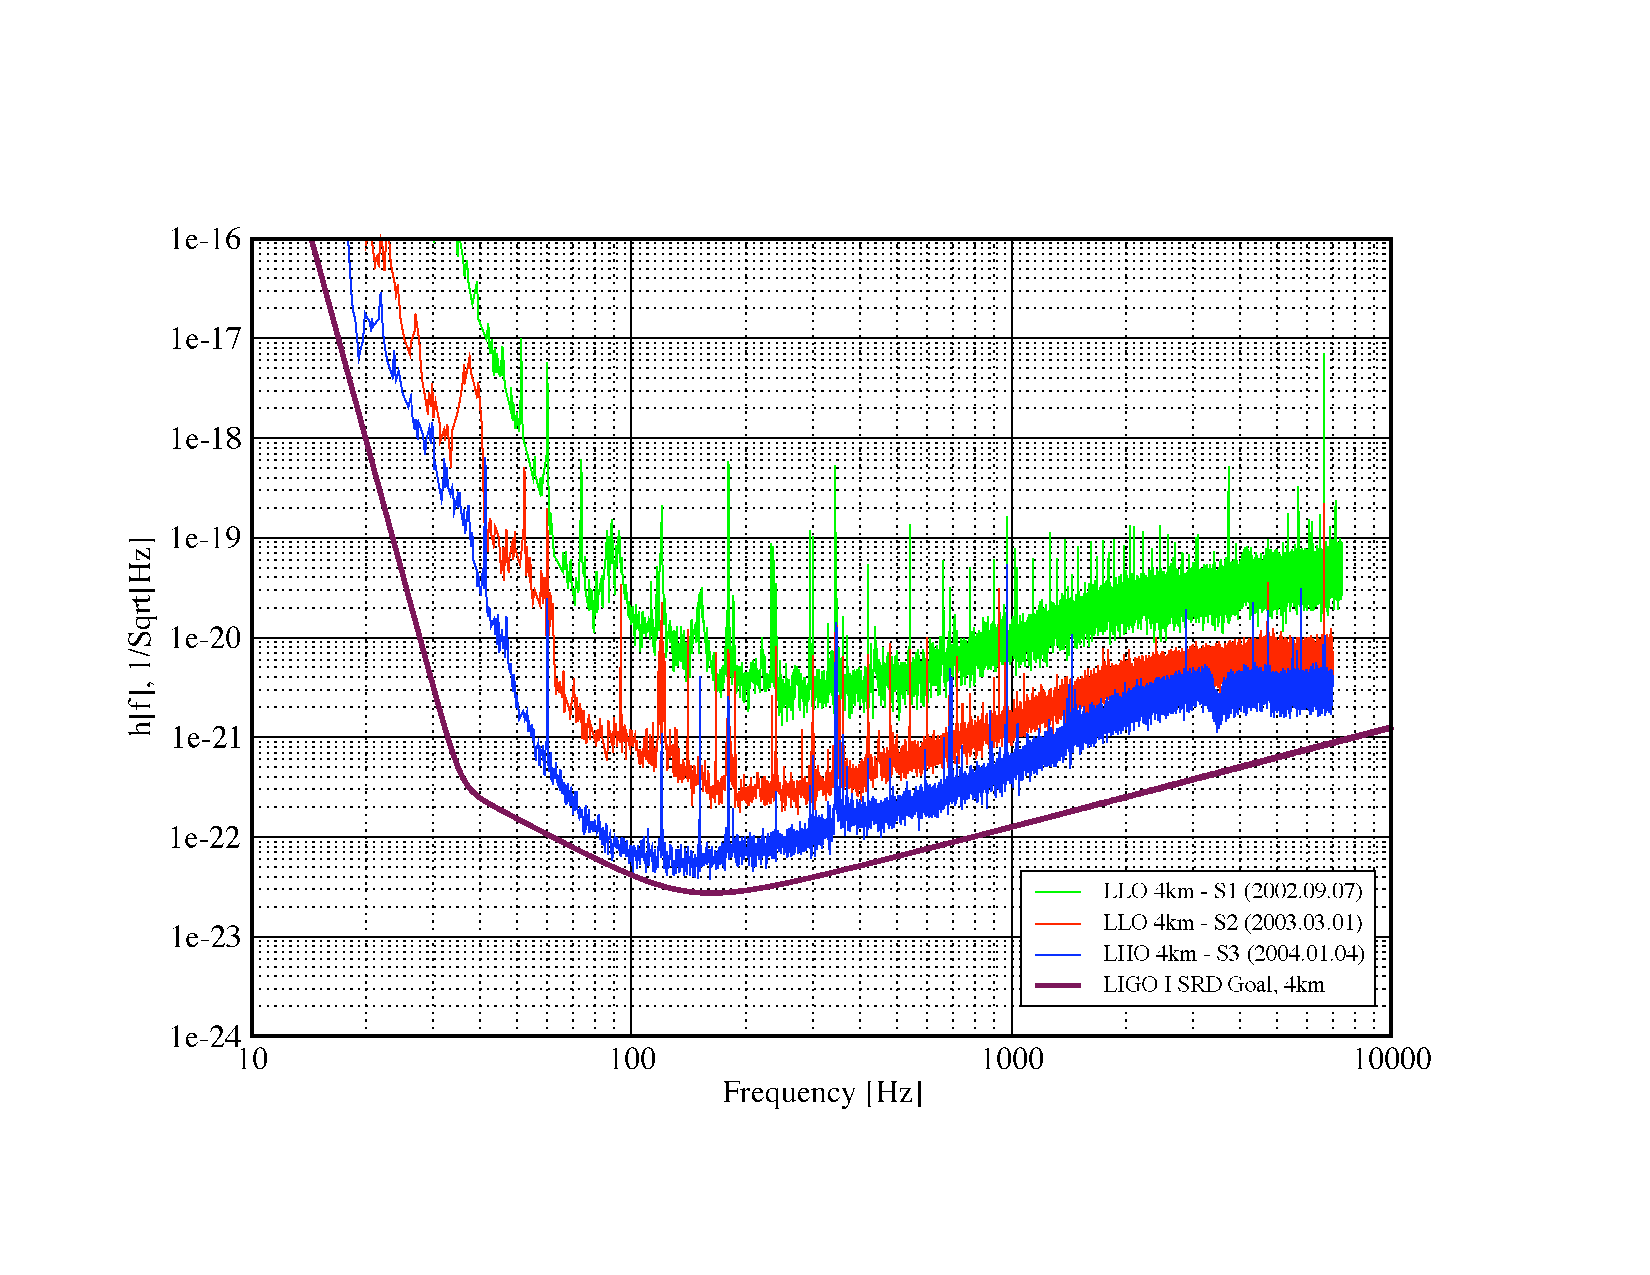
\includegraphics[width=\textwidth]{figures/conclusion/s3strain}
%\end{center}
%\caption[Comparison of Best LIGO Interferometer Sensitivity]{%
%\label{f:s3strain}
%Comparison of the best sensitivities of the LIGO interferometers between
%science runs. The solid curve shows the design sensitivity for the $4$~km
%interferometers: the LHO $4$~km is only a factor of $\sim 2$ away from design
%at $100$~Hz during S3.
%}
%\end{figure}
%
